\documentclass{standalone}
\usepackage{tikz}

\usetikzlibrary{decorations.pathreplacing}

\begin{document}

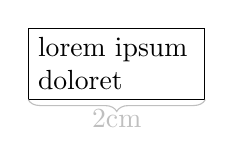
\begin{tikzpicture}
%x description="node with label"
%x step={
\node [text width=2cm, draw] 
	{lorem ipsum doloret};
%x }

	\draw 
		[decorate, decoration={brace, amplitude=0.15cm}, lightgray] 
		(current bounding box.south east) 
		-- node [below] {2cm}
		(current bounding box.south west);
\end{tikzpicture}

\end{document}
